This chapter will show implementation workflow for generating CoreDSL code from OSAL files. We first introduce the overview of the implementation workflow, then we will discuss details of each stage in the workflow. The final part of this chapter will discuss the testing with M2-ISA-R.

\section{Implementation Workflow}

\begin{figure}[ht]
  \centering
  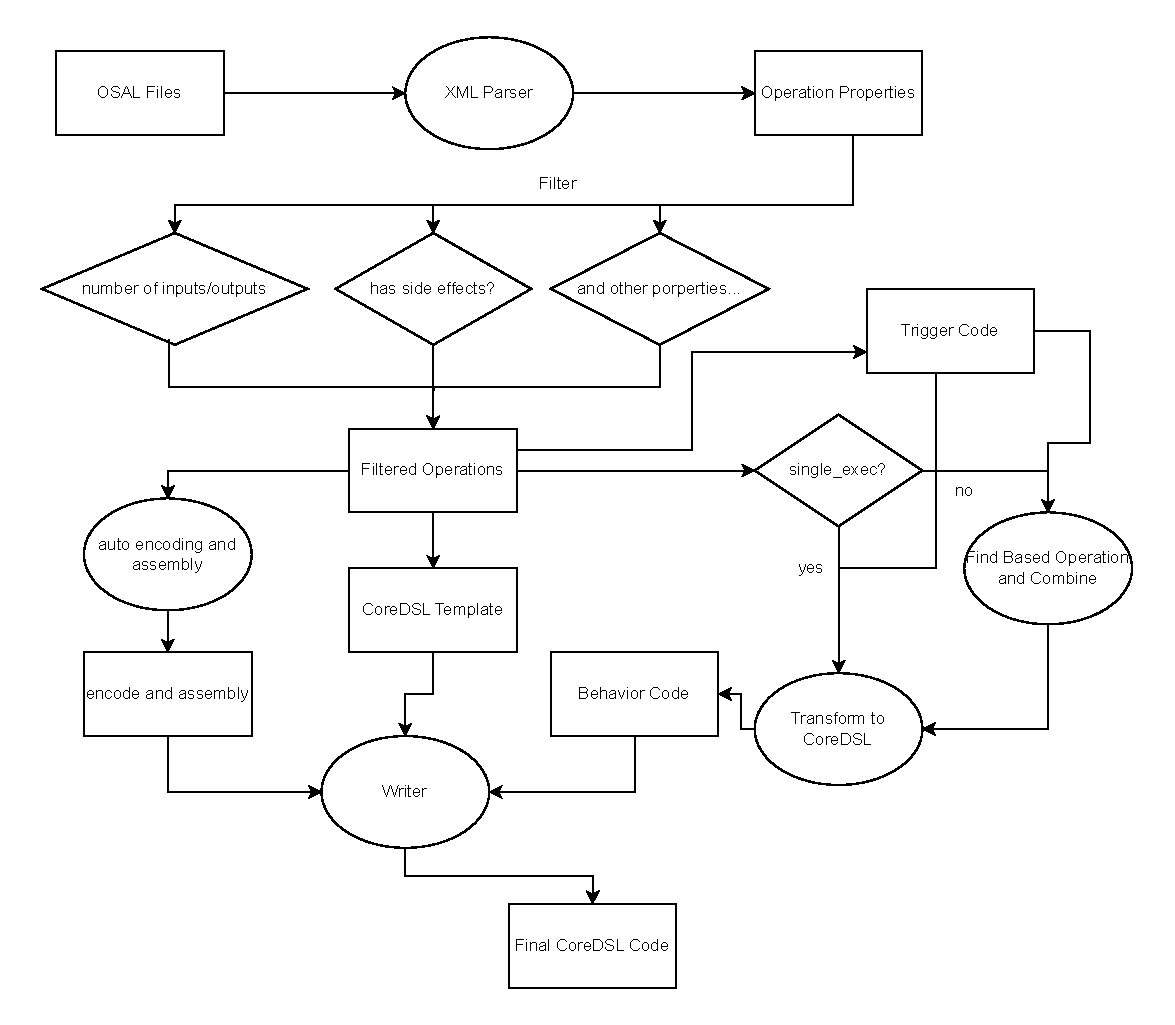
\includegraphics[width=\linewidth]{figures/flow.pdf}
  \caption{Implementation Flow}
  \label{fig:flow}
\end{figure}

The workflow for generating CoreDSL code from OSAL files, as depicted in Fig.~\ref{fig:flow}, involves several key stages that transform input operations into CoreDSL code suitable for integration into M2-ISA-R. The overall flow can be divided into the following steps:

\subsection{OSAL Files}
The process begins with the input OSAL (Operation Set Architecture Language) files, which contain the operation definitions. OpenASIP uses XML and C++ like language to define the properties, semantics and behaviors of custom operations. OSAL files are consisted of the .cc files and .opp files, which are in XML format. The .cc files contain the trigger code for the operations, while the .opp files contain the operation properties and semantics. The description of the properties, semantics and behaviors are in the \textit{OpenASIP User Manual} \cite{openasipmanual}. The following example shows the ADD operation defined in the OSAL files:

\begin{lstlisting}[caption={.opp file Example \cite{openasipcode}},captionpos=b]
// ADD operation properties and semantics in .opp file
<operation>
<name>ADD</name>
<description>Integer addition. Output 3 is sum of inputs 1 and 2.</description>
<inputs>2</inputs>
<outputs>1</outputs>
<in element-count="1" element-width="32" id="1" type="SIntWord">
  <can-swap>
    <in id="2"/>
  </can-swap>
</in>
<in element-count="1" element-width="32" id="2" type="SIntWord">
  <can-swap>
    <in id="1"/>
  </can-swap>
</in>
<out element-count="1" element-width="32" id="3" type="SIntWord"/>
<trigger-semantics>
  EXEC_OPERATION(add, IO(1), IO(2), IO(3));
</trigger-semantics>
</operation>
\end{lstlisting}

\begin{lstlisting}[caption={.cc file Example \cite{openasipcode}},captionpos=b]
// ADD operation trigger code in .cc file
OPERATION(ADD)

TRIGGER
    IO(3) = UINT(1) + UINT(2);
END_TRIGGER;

END_OPERATION(ADD)
\end{lstlisting}

\subsection{XML Parser}

To translate these operations defined in OSAL files in into CoreDSL, we need to parse the XML representation and extract the necessary information. We developed an XML parser based on the pandas package in Python to read the XML files and extract the operation details.

The parser utilizes an object-oriented approach to ensure modularity and scalability. The extracted data is stored in the form of pandas DataFrames, which allows for efficient manipulation and filtering of the operations in the subsequent stages of processing. This structure provides flexibility for further

\subsection{Operation Filtering}

The next stage involves filtering the operations based on predefined criteria. This step is crucial for identifying the operations that are suitable for further processing and transformation into CoreDSL code. The filtering process is designed to select operations that meet specific requirements, such as the number of inputs and outputs, the presence of side effects, or other characteristics that are relevant for the translation process. The filtering criteria are defined based on the properties and semantics of the operations as specified in the XML files. Table~\ref{tab:filtercriteria} shows the filtering criteria used in the implementation.

% Filter Criteria
\begin{table}[hb]
    \centering
    \caption{Operation Filtering Criteria}
    \label{tab:filtercriteria}
    \begin{tabular}{@{}ll@{}}
    \toprule
    \textbf{Properties} & \textbf{Criteria} \\ \midrule
    Minimum Inputs & 0 \\
    Maximum Inputs & 3 \\
    Minimum Outputs & 0 \\
    Maximum Outputs & 1 \\
    Element Widths & [1, 5, 8, 16, 32] \\
    No Control Flow & False \\
    No Call & False \\
    No Branch & False \\
    Element Count 1 & False \\
    No Side Effects & False \\
    No Memory Reads & False \\
    No Memory Writes & False \\
    No HalfFloatWord & False \\
    No FloatWord & False \\
    No RawData & False \\ \bottomrule
    \end{tabular}
\end{table}

\subsection{CoreDSL Template Generation}

The generation of the CoreDSL template involves several key steps. First, an empty CoreDSL template is created, which serves as the scaffold for defining the behavior of the custom operations. Then, the program iterates over the filtered operations and fills in the necessary details into the template. The generation process leverages the parsed information from the XML files, including operation-specific attributes such as the number of input and output registers. The custom instructions are automatically encoded based on their properties, and the corresponding assembly code is generated.

\begin{lstlisting}[caption={CoreDSL Template},captionpos=b]
InstructionSet OpenASIP_base extends RV32I {
  functions{
      // Inline functions for behavior
  }
  instructions {
      // Example for custom instruction
      OpenASIP_{filename}_{operation_name} {
          encoding: // Encoding will be generated here
          assembly: // Assembly code will be generated here
          behavior: {
              // Behavior code will be generated here
          }
      }
      // Additional instructions will be iteratively generated
  }
}
\end{lstlisting}

\subsubsection{Inline Function}

The inline functions required for custom operations are defined as part of the \textit{trigger codes} within the OpenASIP framework. Although OpenASIP provides the trigger code definition, it does not include the actual implementation of these inline functions. Fortunately, these functions are relatively simple to implement and are inserted at the beginning of the CoreDSL file. This ensures that all behavior code for custom instructions can utilize these functions during execution. The following example demonstrates how inline functions are defined in the CoreDSL template:

\begin{lstlisting}
// Returns the minimum of two signed integers.
signed<32> min(signed<32> a, signed<32> b) [[inline]] {
    return (a < b) ? a : b;
}
\end{lstlisting}

\subsubsection{Auto Encoding and Assembly}

The encoding process for custom instructions is handled automatically by the program. As the filtered operations are processed sequentially, each instruction is assigned an encoding that follows the RISC-V extension format. For example, instructions with two input registers (\textbf{rs1} and \textbf{rs2}) and one output register (\textbf{rd}) will be encoded in a standard 32-bit RISC-V format R-type instruction. Here is an example of how the encoding is generated:

\begin{lstlisting}
encoding: 7'b0000000 :: rs2[4:0] :: rs1[4:0] :: 3'b000 :: rd[4:0] :: 7'b0001011;
\end{lstlisting}

For assembly code generation, the program analyzes the XML-defined instruction attributes, such as the number of source and destination registers. Based on these attributes, it generates the corresponding assembly format string, ensuring that the generated assembly matches the intended behavior of each instruction. The following example shows how the registers are referenced in the assembly code:

\begin{lstlisting}
assembly: "{name(rd)}, {name(rs1)}, {name(rs2)}";
\end{lstlisting}

This ensures that all operations are properly defined within the CoreDSL framework, both at the encoding level and in terms of their assembly representation.

\subsection{Behavior Code Generation}

The generation of behavior code for custom operations is a crucial step in translating operation semantics into executable instructions within the CoreDSL framework. This process primarily revolves around interpreting the trigger semantics provided for each operation and converting them into behavior code that can be executed by the target architecture.

% How to classify operations as single_exec_operation
% non_single_exec_operation
\begin{lstlisting}[caption={Non-Single Exec Operation Semantics Example},captionpos=b]
SimValue shifted;
EXEC_OPERATION(shl, IO(1), 1, shifted);
EXEC_OPERATION(add, shifted, IO(2), IO(3));
\end{lstlisting}
% single_exec_operation
\begin{lstlisting}[caption={Single Exec Operation Semantics Example},captionpos=b]
EXEC_OPERATION(add, IO(1), IO(2), IO(3));
\end{lstlisting}

The behavior code generation process in this framework involves two main types of operations: \textbf{single\_exec\_operation} and \textbf{non\_single\_exec\_operation} operations. The approach to generating behavior code differs depending on the type of operation, and the handling of each is described below.

\subsubsection{Handling \textbf{single\_exec\_operation}}

For operations classified as single, which involve exactly zero or one \textbf{EXEC\_OPERATION}, the process is relatively straightforward. The trigger code for these operations is directly searched within the parsed XML file, and once found, it is transformed into behavior code for the CoreDSL template.

\begin{enumerate}
    \item \textbf{Search for Trigger Code}: The system directly locates the corresponding trigger code for the operation. If the trigger code is found, it is translated and formatted according to the CoreDSL behavior syntax.

    \item \textbf{Behavior Code Translation}: The translation process involves adjusting the variable names and formatting to conform to the CoreDSL standard. For instance, custom register names are transformed into the CoreDSL format using \textbf{X[rs1]}, \textbf{X[rs2]}, and \textbf{X[rd]}.

    \item \textbf{Example}:
    \begin{lstlisting}
// Translated behavior code for a single_exec_operation
X[rd % RFS] = X[rs1 % RFS] + X[rs2 % RFS]; // Simple addition
    \end{lstlisting}
\end{enumerate}

\subsubsection{Handling \textbf{Non-single\_exec\_operation} Instructions}

For operations that are not classified as \textbf{single\_exec\_operation}, OpenASIP does not provide a direct trigger code. Instead, the process requires extracting relevant properties from the XML representation and using those properties to identify the appropriate base operations (\textbf{based operations}). The steps for handling these more complex operations are as follows:

\begin{enumerate}
    \item \textbf{Extract Properties from XML}: The first step is to parse the XML file and extract key properties such as the number of inputs (\textbf{rs}) and outputs (\textbf{rd}), as well as other operation-specific semantics that define the behavior of the instruction.

    \item \textbf{Identify Based Operations}: Once the necessary properties are extracted, the system searches for related base operations (\textbf{EXEC\_OPERATION}) that can be combined to define the full behavior of the instruction. These base operations may consist of multiple execution steps, each of which contributes to the final instruction's functionality.

    \item \textbf{Combining Based Operations}: If multiple base operations are found, they are combined sequentially in the generated behavior code. Each base operation's trigger code is retrieved, transformed, and concatenated to form the full behavior.

    \item \textbf{Example}:
    \begin{lstlisting}
// Combined behavior code from multiple based operations
signed<32> shifted = X[rs1 % RFS] << 1;  // First base operation: shift left
X[rd % RFS] = shifted + X[rs2 % RFS];    // Second base operation: addition
    \end{lstlisting}

    \item \textbf{Modifying Variable Names}: Based on the extracted input-output properties, the system adjusts the variable names in the behavior code to align with the correct registers. The next section will discuss how variable names are handled in more detail.
\end{enumerate}

\subsubsection{Handling Different Variable Names}

In some cases, variable names in the trigger code might differ from the expected format used in the CoreDSL framework. This is a common issue, especially when operations are defined in different contexts or environments. The tool handles this issue by:

\begin{enumerate}
    \item \textbf{Pattern Matching and Variable Mapping}: The tool applies pattern matching to identify variables in the trigger code (e.g., \textbf{UINT(1)}, \textbf{SIntWord}, \textbf{IO(3)}) and maps them to the expected format used in the target architecture. This ensures consistency in variable naming across all operations.

    \item \textbf{Renaming Strategy}: If the trigger code uses custom variable names (e.g., \textbf{temp\_reg}), the tool automatically replaces these with the standard naming convention used in CoreDSL . This is done using regular expressions to match and substitute variable names accordingly.

    \item \textbf{Example}:
    \begin{lstlisting}
// Before transformation: uses custom variable names
SIntWord in1 = static_cast<SIntWord>(UINT(1));
SIntWord in2 = static_cast<SIntWord>(UINT(2));
IO(3) = (in1 > in2) ? 1 : 0;

// After transformation: standard variable names
signed<32> in1 = (signed<32>)(X[rs1 % RFS]);
signed<32> in2 = (signed<32>)(X[rs2 % RFS]);
X[rd % RFS] = (in1 > in2) ? 1 : 0;
    \end{lstlisting}
\end{enumerate}

This automatic renaming ensures that all behavior code conforms to the same format, regardless of the original trigger code's naming conventions.

\subsubsection{Handling Other Corner Cases}

In addition to the common cases mentioned above, the tool also addresses several corner cases that may arise during behavior code generation:

\begin{enumerate}
    \item \textbf{Multiple \textbf{EXEC\_OPERATION} Cases}: In this case, the tool concatenates the behavior of these operations, ensuring that all steps are executed in the correct order. For example, if an operation involves both a shift and an addition, the tool ensures that both operations are included in the final behavior code.

    \item \textbf{Complex Trigger Semantics}: For operations with complex trigger semantics (e.g., involving multiple registers or advanced arithmetic operations), the tool decomposes the trigger code into manageable steps and generates the corresponding behavior code. This may involve splitting a single line of code into multiple steps to ensure clarity and correctness.

    \item \textbf{Error Handling}: In situations where runtime errors are defined (e.g., division by zero), the tool ensures that appropriate error handling mechanisms are inserted into the behavior code. This includes raising errors or returning safe default values when an error condition is detected.
\end{enumerate}

\subsubsection{Final Behavior Code Generation}

The final behavior code is generated by combining the transformed trigger code for \textbf{single\_exec\_operation} or the combined base operations for \textbf{non\_single\_exec\_operation} instructions. This ensures that each operation is fully defined within the CoreDSL framework and can be executed correctly on the target architecture.

The behavior code is then inserted into the CoreDSL template, completing the generation process for each custom instruction.

\begin{lstlisting}
// Example of final behavior code for a combined operation
// Arithmetic shift right (sign bit duplicated). Input 1 is value to be shifted and input 2 is shift amount. Output 3 is result from operation.
signed<32> int1 = (signed<32>)(X[rs1 % RFS]);
signed<32> int2 = (signed<32>)(X[rs2 % RFS]);
// Check if shift amount is greater than minimum of register width and 32
if (int2 > min(
        (signed<32>)(BWIDTH(X[rs1 % RFS])),
        (signed<32>)(32))) {
    X[rd % RFS] = 0;
}

signed<32> int3 = int1 >> int2;
X[rd % RFS] = (signed<32>)(int3);
\end{lstlisting}

By handling both simple and complex cases, this approach ensures that the generated behavior code is both comprehensive and tailored to the specific needs of each instruction.

\subsection{Code Generation}

The final stage of the implementation workflow involves generating the complete CoreDSL code for the custom instruction set. This process combines the CoreDSL template with the behavior code for each custom operation, resulting in a fully defined instruction set that can be integrated into the M2-ISA-R architecture.

\section{Test with M2-ISA-R}

During the development process, M2-ISA-R was utilized to verify the correctness of the generated CoreDSL code and identify potential issues. M2-ISA-R provides a comprehensive framework for testing the functionality of custom instruction sets by parsing the CoreDSL and generating the corresponding ETISS plugins.

\subsection{Error Detection}

Throughout the code generation phase, M2-ISA-R was used to validate the syntax and semantics of the generated CoreDSL instructions. The tool was instrumental in identifying errors related to:

\begin{itemize}
    \item \textbf{Syntax Errors}: M2-ISA-R automatically checks for syntax inconsistencies within the CoreDSL files. Any improperly formatted code, missing keywords, or incorrect structure was flagged for correction.
    \item \textbf{Behavioral Semantics}: M2-ISA-R also validated the behavior code for each instruction, ensuring that the execution semantics were correctly translated from the original XML description.
    \item \textbf{Variable Mismatches}: Issues related to incorrect variable naming or mismatches between input-output registers were quickly detected, allowing for prompt corrections in the code generation process.
\end{itemize}

Each time an issue was identified by M2-ISA-R, the error messages provided guidance on where and how the problem could be resolved. This allowed for an iterative process where code could be quickly corrected based on the tool's feedback.

\subsection{Iterative Debugging and Error Resolution}

As errors were identified, corrections were made iteratively:

\begin{enumerate}
    \item \textbf{Syntax Corrections}: Syntax errors, such as missing semicolons, misplaced braces, or improperly formatted CoreDSL code, were corrected immediately after detection.
    \item \textbf{Behavior Code Adjustments}: If M2-ISA-R detected inconsistencies in the behavior code, such as incorrect execution semantics or uninitialized variables, the tool provided clear feedback that allowed for prompt adjustments. This was particularly useful for ensuring that complex instructions with multiple base operations were executed in the correct sequence.
    \item \textbf{Refinement of Variable Names}: In some cases, variable names in the behavior code did not match the expected register format. M2-ISA-R provided error messages that pointed out these mismatches, prompting revisions in the generated code to ensure that input and output registers were correctly assigned.
\end{enumerate}

\subsection{Final Code Generation for ETISS}

After resolving all detected errors, M2-ISA-R was used to generate the final ETISS plugin. The tool parsed the corrected CoreDSL code and produced the necessary architecture plugin for ETISS. This plugin was then integrated into the ETISS framework, allowing the custom instruction set to be simulated and tested within a realistic RISC-V environment.

The use of M2-ISA-R ensured that the CoreDSL code was syntactically correct, semantically meaningful, and fully compatible with ETISS. This iterative testing and debugging process was crucial for developing a robust and error-free instruction set.

\subsection{Testing with ETISS}

With the ETISS plugin generated by M2-ISA-R, the custom instruction set was ready for testing. ETISS was used to simulate the instruction set on various machine learning models and workloads, allowing for performance evaluation and validation of the custom extensions.

The final tests confirmed that the generated instructions were executed correctly within ETISS, and performance metrics were collected for further analysis.
